\section{Backpropagation}
\subsection*{Big Picture}
\begin{itemize}
    \item In ANNs, we learn both $f$ and $\boldsymbol{\theta}$, meaning that the log loss is not convex
    \item Backpropagation uses the chain rule in combination with dynamic programming techniques to compute the gradient of the log loss $\nabla_{\boldsymbol{\theta}} L(\boldsymbol{\theta})$
\end{itemize}

{\color{black}\hrule height 0.001mm}

\subsection*{Point of Departure}

\emph{Composite function} --- Ordered series of equations (\emph{primitives}), where each equation is a function only of the preceding equations. E.g.:
$
f(x, z) = x^2 + 3z, \quad \textrm{with }
a = x^2, \quad b = 3z, \quad c = a + b, \quad f(x, z) = c
$

{\color{lightgray}\hrule height 0.001mm}

\emph{Computation graph $\mathcal{G}$} --- Graphical representation of a composite function
\begin{itemize}
    \item \emph{Directed acyclic hypergraph} $(E, V)$ where $V$ is the set of vertices (nodes) representing variables and $E$ is the set of edges representing functions
    \begin{itemize}
        \item Directed: One direction
        \item Acyclic: No cycles
        \item An edge can connect any number of vertices, not just two
    \end{itemize}
    \item Edge from $v' \to v$: labeled with a differentiable function $f_v$
    \item Vertex $v$ with outgoing edges: argument to $f_v$
    \item Vertex $v$ with incoming edges: result of $f_v$
    \item If we have $n$ input nodes and $|E| = M$ edges, we have $|V| = M + n$ total nodes
\end{itemize}

{\color{lightgray}\hrule height 0.001mm}

\emph{Bauer's Formula} ---
\begin{itemize} 
    \item For two nodes $z_i$ and $z_j$ in $\mathcal{G}$, let the Bauer path $P(i, j)$ define the set of all directed paths starting at $j$ and ending at $i$
    \item Partial derivative:
    $
    \frac{\partial z_i}{\partial z_j} = \sum_{p \in P(j, i)} \prod_{(k, l) \in p} \frac{\partial z_l}{\partial z_k}
    $ where we sum over all paths and take the product over all nodes on a given path\\
    Proof:
    \begin{itemize}
        \item Base case:$i = j$, i.e., $z_i = z_j$:
        $\frac{\partial z_i}{\partial z_j} = 1$
        \item Inductive hypothesis: Bauer's formula holds for all $j \leq i$
        \item Inductive step:
        \begin{itemize}
            \item Let $m < j$ (i.e., $z_m$ comes before $z_j$ in topological order, and $j \in \textrm{out}(m)$)
            \item $
            \frac{\partial z_i}{\partial z_m} = \sum_{j \in \textrm{out}(m)} \frac{\partial z_i}{\partial z_j} \frac{\partial z_j}{\partial z_m}
            $ by the chain rule
            \item $
            \frac{\partial z_i}{\partial z_m} = \sum_{j \in \textrm{out}(m)} (\sum_{p \in P(j, i)} \prod_{(k, l) \in p} \frac{\partial z_l}{\partial z_k}) \frac{\partial z_j}{\partial z_m}
            $ due to inductive hypothesis
            \item $
            \frac{\partial z_i}{\partial z_m} = \sum_{j \in \textrm{out}(m)} (\sum_{p \in P(j, i)} \frac{\partial z_j}{\partial z_m} \prod_{(k, l) \in p} \frac{\partial z_l}{\partial z_k})
            $ due to distributivity
            \item $
            \frac{\partial z_i}{\partial z_m} = \sum_{p \in P(m, i)} \prod_{(k, l) \in p} \frac{\partial z_l}{\partial z_k}
            $ by concatenating paths
        \end{itemize}
    \end{itemize}
    \item Challenge of naively calculating this: With $\sum_{p \in P(j, i)}$, we are summing over an exponential number of paths, leading to a runtime complexity of $O(|P(j, i)|) = O(2^{|E|})$ 
\end{itemize} 

{\color{black}\hrule height 0.001mm}

\subsection*{Forward Pass}
Compute output of $f$ by randomly initializing values of input nodes:
\begin{enumerate}
    \item Initialize node values:
    $
    z_i =
    \begin{cases}
    x_i & \textrm{if } i \leq n \quad (\textrm{n input nodes}) \\
    0 & \textrm{if } i > n \quad (\textrm{non-input nodes})
    \end{cases}
    $For $i = n+1, \dots, M$ non-input nodes:
    $
    z_i = g_i\big(\langle z_{\textrm{pa}(i)} \rangle\big)
    $
    where $g_i$ denotes the primitive at edge $i$ and $\langle z_{\textrm{pa}(i)} \rangle$ denotes the ordered set of parent nodes of $z_i$
    \item Return $\{z_1, z_2, \dots, z_M\}$
\end{enumerate}
Properties:
\begin{itemize}
    \item Runtime complexity: $O(|E|)$, i.e., linear in the number of edges
    \item Space complexity: $O(|V|)$, i.e., linear in the number of vertices
\end{itemize}

{\color{black}\hrule height 0.001mm}

\subsection*{Backpropagation}
After forward pass, compute the gradient of $f$ with respect to input nodes:
\begin{enumerate}
    \item Perform forward pass: $\boldsymbol{z} \gets \textrm{forward propagate}(f, \boldsymbol{x})$
    \item Initialize:
    $
    \frac{\partial f}{\partial z_i} =
    \begin{cases}
    1 & \textrm{if } i = M\\
     & (\textrm{gradient of } f \textrm{ with respect to}\\
     & \textrm{output node = 1, since } \partial f / \partial f = 1)\\
    0 & \textrm{otherwise}
    \end{cases}
    $
    \item For $i = M-1, \dots, 1$:
    $
    \frac{\partial f}{\partial z_i} = \sum_{j:i \in \textrm{Pa}(i)} \frac{\partial f}{\partial z_j} \frac{\partial z_j}{\partial z_i} = \sum_{j:i \in \textrm{Pa}(i)} \frac{\partial f}{\partial z_j} \frac{g_j\big(\langle z_{\textrm{pa}(j)} \rangle\big)}{\partial z_i}
    $
    \item Return $\left[ \frac{\partial f}{\partial z_1}, \frac{\partial f}{\partial z_2}, \dots, \frac{\partial f}{\partial z_M} \right]$
\end{enumerate}
Properties:
\begin{itemize}
    \item Improvement over Bauer's formula: Partial derivatives that appear on multiple paths are memoized
    \item Runtime complexity: $O(|E|)$, i.e., the same as forward pass
    \item Space complexity: $O(|V|)$, i.e., the same as forward pass
    \item \emph{Cheap gradient principle}: Calculating the gradient has the same complexity as evaluating the function
\end{itemize}
Extension of backpropagation to $k^{th}$ order derivatives:
\begin{itemize}
    \item Backpropagation on a graph with $|E|$ edges, for inputs $\boldsymbol{x} = (x_1, \dots, x_n)^\intercal$, for the $k^{th}$ order derivative has runtime $\mathcal{O}(|E|n^{k-1})$\\
    Proof:
    \begin{itemize}
        \item For second-order derivative: $
        \nabla_2 f(\boldsymbol{x}) \textrm{(i.e. Hessian)} = 
        \begin{bmatrix}
        \nabla( \boldsymbol{e}_1^\intercal \nabla f(\boldsymbol{x}) \textrm{(i.e. Jabobian)})\\
        ...\\
        \nabla( \boldsymbol{e}_n^\intercal \nabla f(\boldsymbol{x}))
        \end{bmatrix}
        $ because $\boldsymbol{e}_k^\intercal \boldsymbol{A}$ returns $k^{th}$ row of $\boldsymbol{A}$
        \item For third-order derivative, similar principle
        \item We first differentiate in $M$ edges ($\nabla_1$), which means complexity is $1 \times M$
        \item We then differentiate by $n$ variables in $M$ edges ($\nabla_2$), which means complexity is $n \times M$
        \item We then differentiate these $n$ variables by another $n$ variables in $M$ edges ($\nabla_3$), which means complexity is $n^2 \times M$
        \item $...$
    \end{itemize}
\end{itemize}
Requirements for backpropagation:
\begin{itemize}
    \item Weights need to be initialized to different values: If they are initialized to the same constant, during backpropagation, all neurons receive the same gradient updates
    \begin{itemize}
        \item Weights initialized to $0$:
        \begin{itemize}
            \item $\boldsymbol{h} = \varphi\left( \boldsymbol{x} \boldsymbol{B}^{[1]}\right) = 0$ where $\boldsymbol{h}$ corresponds to $z$, $\varphi$ is the primitive, and $\boldsymbol{x}$ corresponds to the input nodes 
            \item $\boldsymbol{y} = \boldsymbol{h} \boldsymbol{B}^{[2]} = 0$ where $\boldsymbol{y}$ corresponds to $z'$
            \item $\frac{\partial L}{\partial \boldsymbol{B}^{[2]}} = \frac{\partial L}{\partial \boldsymbol{y}} \frac{\partial \boldsymbol{y}}{\partial \boldsymbol{B}^{[2]}} = \frac{\partial L}{\partial \boldsymbol{y}} \boldsymbol{h} = 0$, i.e. $\boldsymbol{B}^{[2]}$ is not updated
            \item $\frac{\partial L}{\partial \boldsymbol{B}^{[1]}} = \frac{\partial L}{\partial \boldsymbol{y}} \frac{\partial \boldsymbol{y}}{\partial \boldsymbol{h}} \frac{\partial \boldsymbol{h}}{\partial \boldsymbol{B}^{[1]}} = \frac{\partial L}{\partial \boldsymbol{y}} \boldsymbol{B}^{[2]} \frac{\partial \boldsymbol{h}}{\partial \boldsymbol{B}^{[1]}} = 0$, i.e. $\boldsymbol{B}^{[1]}$ is not updated
            \item Thus, weights will always remain $0$ and network will not learn
        \end{itemize}
        \item Weights initialized to same constant:
        \begin{itemize}
            \item $\boldsymbol{B}^{[1]} = \boldsymbol{B}^{[2]}$
            \item $\boldsymbol{h}_1 = \boldsymbol{h}_2$
            \item $\frac{\partial L}{\partial \boldsymbol{B}^{[1]}} = \frac{\partial L}{\partial \boldsymbol{B}^{[2]}}$
            \item Thus, weights will always receive same updates, will remain equal, and network will not learn
        \end{itemize}
    \end{itemize}
    \item At least one activation must be non-linear so that there is a non-zero gradient
\end{itemize}

\begin{multicols}{2}
\textit{1) Forward pass and backpropagation in graph}\\
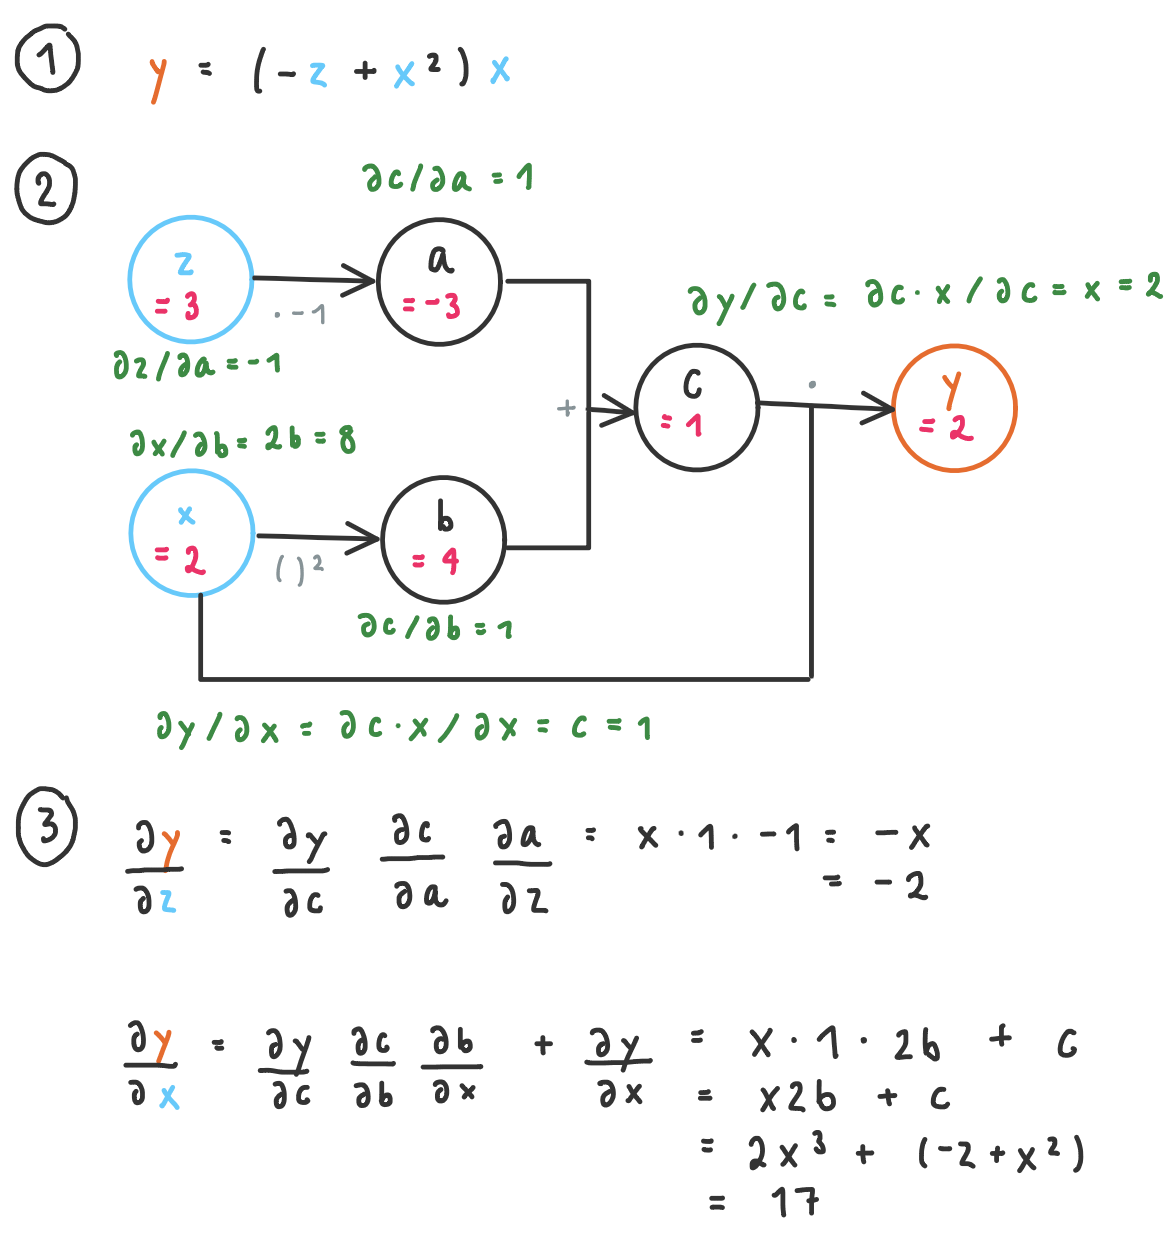
\includegraphics[height=25mm]{inhalt/images/NLP/05_backpropagation_1.png}
\end{multicols}